%%%% ijcai24.tex

\typeout{IJCAI--24 Instructions for Authors}

% These are the instructions for authors for IJCAI-24.

\documentclass{article}
\pdfpagewidth=8.5in
\pdfpageheight=11in

% The file ijcai24.sty is a copy from ijcai22.sty
% The file ijcai22.sty is NOT the same as previous years'
\usepackage{ijcai24}

% Use the postscript times font!
\usepackage{times}
\usepackage{soul}
\usepackage{url}
\usepackage[hidelinks]{hyperref}
\usepackage[utf8]{inputenc}
\usepackage[small]{caption}
 
 %package to manage images
\usepackage{graphicx}
\graphicspath{ {./results/} }

\usepackage{amsmath}
\usepackage{amsthm}
\usepackage{booktabs}
\usepackage{algorithm}
\usepackage{algorithmic}
\usepackage[switch]{lineno}


%für symbols
\usepackage{dsfont}
\usepackage{amssymb}


% Comment out this line in the camera-ready submission
%\linenumbers

\urlstyle{same}

% the following package is optional:
%\usepackage{latexsym}

% See https://www.overleaf.com/learn/latex/theorems_and_proofs
% for a nice explanation of how to define new theorems, but keep
% in mind that the amsthm package is already included in this
% template and that you must *not* alter the styling.
\newtheorem{example}{Example}
\newtheorem{theorem}{Theorem}

% Following comment is from ijcai97-submit.tex:
% The preparation of these files was supported by Schlumberger Palo Alto
% Research, AT\&T Bell Laboratories, and Morgan Kaufmann Publishers.
% Shirley Jowell, of Morgan Kaufmann Publishers, and Peter F.
% Patel-Schneider, of AT\&T Bell Laboratories collaborated on their
% preparation.

% These instructions can be modified and used in other conferences as long
% as credit to the authors and supporting agencies is retained, this notice
% is not changed, and further modification or reuse is not restricted.
% Neither Shirley Jowell nor Peter F. Patel-Schneider can be listed as
% contacts for providing assistance without their prior permission.

% To use for other conferences, change references to files and the
% conference appropriate and use other authors, contacts, publishers, and
% organizations.
% Also change the deadline and address for returning papers and the length and
% page charge instructions.
% Put where the files are available in the appropriate places.


% PDF Info Is REQUIRED.

% Please leave this \pdfinfo block untouched both for the submission and
% Camera Ready Copy. Do not include Title and Author information in the pdfinfo section
\pdfinfo{
/TemplateVersion (IJCAI.2024.0)
}

\title{White-Box vs Black-Box Methods: A Comparative Study on Explaining DNNs}


% Single author syntax
\author{
    Tom Backert
    \affiliations
    University of Luebeck, Luebeck, Germany\\
    Institute for Software Engineering und Programming Languages
    \emails
    tom.backert@student.uni-luebeck.de
}

% Multiple author syntax (remove the single-author syntax above and the \iffalse ... \fi here)
\iffalse
\author{
First Author$^1$
\and
Second Author$^2$\and
Third Author$^{2,3}$\And
Fourth Author$^4$\\
\affiliations
$^1$First Affiliation\\
$^2$Second Affiliation\\
$^3$Third Affiliation\\
$^4$Fourth Affiliation\\
\emails
\{first, second\}@example.com,
third@other.example.com,
fourth@example.com
}
\fi

% Here starts the main part of the paper
\begin{document}

\maketitle

\begin{abstract}
    As deep neural networks (DNNs) become increasingly integral to various fields, understanding their decision-making processes is paramount. Explainable Artificial Intelligence (XAI) methods, specifically feature importance techniques, are essential tools for enhancing the interpretability of these complex models. This paper presents a comparative study of white-box and black-box XAI methods, focusing on Grad-CAM (white-box) and LIME (black-box) as representatives of their respective categories. We explore the trade-offs between these methods in terms of interpretability, fidelity, and computational efficiency. By evaluating their performance using the Explanation Selectivity metric, this study provides insights into the suitability of these methods for object recognition tasks. The findings aim to guide the selection of appropriate XAI methods, contributing to the development of more transparent and trustworthy AI systems.
\end{abstract}

\section{Introduction}
\subsection{Motivation and Practical Goal}
As Artificial Intelligence (AI) models become increasingly complex, it becomes harder for humans to understand these systems. This is particularly true in fields like computer vision, where Deep Neural Networks (DNNs) often function as black-box models, leading even experts to lose track of their inner workings. This highlights the critical importance of developing methods to explain AI model decisions.

Explainable Artificial Intelligence (XAI) aims to make AI models more interpretable and understandable for humans. XAI seeks to bridge the gap between the opaque nature of traditional AI models and the need for transparency and accountability in decision-making processes. This is especially crucial in high-stakes domains such as healthcare, finance, and autonomous systems like self-driving cars, where decisions can significantly impact people’s lives.

By identifying potential biases, errors, or areas for optimization, XAI can help improve AI models. Understanding how models make predictions allows us to better identify and address issues that may lead to inaccurate or unfair outcomes, potentially causing substantial harm. Additionally, XAI can facilitate better collaboration between humans and AI systems by providing explanations that enable humans to understand the rationale behind AI’s suggestions, thereby making informed decisions.

Overall, XAI is essential for ensuring the responsible and safe use of AI systems. It is relevant across all areas of AI and will play a crucial role in ensuring transparency, accountability, and the integration of AI models into society as they continue to evolve.



\subsection{Problem Statement}
% The Case for Explanability
As AI models become more integrated into our daily lives, understanding the factors influencing their decisions becomes increasingly important. This need has driven researchers to focus on developing explainability methods for complex models. However, selecting an appropriate XAI method for a specific application remains a challenge.

% The Case for Feature Importance in Explanability
Although there is a vast array of XAI methods available (see Related Work), this paper focuses specifically on Feature Importance methods due to their critical role in identifying which features are most influential in the model’s predictions. This is essential for building trust in AI systems and facilitating informed decision-making. However, the selection of the appropriate Feature Importance method itself poses significant problems:

\begin{enumerate}
    \item Interpretability vs. Fidelity:
    Balancing interpretability and fidelity is challenging. Interpretability ensures that users can understand the explanations, while fidelity ensures that the explanations accurately reflect the model’s behavior. High interpretability often comes at the cost of fidelity and vice versa.
    \item Black-Box vs. White-Box Methods:
    Deciding between black-box and white-box methods for Feature Importance is complex. Black-box methods, like LIME, do not require access to the model’s internal structure but may lack the depth of explanation provided by white-box methods, like Grad-CAM, which utilize the model’s internal gradients and architecture.
    \item Local vs. Global Explanations:
    Feature Importance methods typically provide local explanations, focusing on specific predictions rather than the model’s overall behavior. This localized focus can limit the broader understanding of the model’s decision-making process.
\end{enumerate}

Given these challenges, it is crucial to understand the trade-offs involved in selecting the appropriate Feature Importance method. An analysis of black-box and white-box Feature Importance methods for local explanations can provide valuable insights into these trade-offs, thereby aiding in making well-informed decisions, and ultimately enhancing trust in AI models, as they become omnipresent in our lives.



\subsection{Scientific Contributions}
% Overarching Research Question
This paper addresses the overarching question: How can an appropriate explanation method (XAI method) be selected for a given application? To answer this, the paper explores two specific sub-questions:

% Subquestions for Paper
\begin{itemize}
    \item Based on which metrics and criteria can a method be selected? (Review section in Background)
    \item What are the advantages and disadvantages of white-box and black-box methods for the application of object recognition? (Application study in Comparison)
\end{itemize}

By examining these questions, this paper aims to provide a comprehensive comparison of white-box and black-box methods, highlighting their suitability and relevance for different use cases.

\subsection{Focus}

The goal of this paper is to compare white-box and black-box methods, specifically focusing on feature importance techniques. To simplify the comparison, one exemplary method from each category was chosen. Specifically, this paper compares LIME (Local Interpretable Model-Agnostic Explanations) ~\cite{ribeiro2016why} as an example of a black-box method and Grad-CAM (Gradient-weighted Class Activation Mapping) ~\cite{Selvaraju_2019} as an example of a white-box method.


% Should be included in the fully researched version
%\section{Related Work}
%\subsection{Context}
%\subsection{Comparison}
%\subsection{Differentiation}

\section{Background}

\subsection{Fundamentals of XAI}


%Functional Description
Explainable Artificial Intelligence (XAI) aims to make AI models more interpretable and understandable to humans. This is crucial for building trust, ensuring transparency, and facilitating decision-making in critical areas such as healthcare, finance, and autonomous systems. XAI techniques can be broadly categorized into two main approaches: white-box methods and black-box methods.

%General Idea
White-box methods rely on an understanding of the internal workings of the AI model to generate explanations. In contrast, black-box methods do not require prior knowledge of the model’s internal structure. Instead, they treat the model as a black box and focus on analyzing its input-output behavior to generate explanations. This approach is particularly useful for complex models such as deep neural networks (DNNs), where understanding the internal workings is challenging or impractical.

%Detailed Explanation
\subsubsection{White-Box Methods}
White-box methods rely on an understanding of the internal workings of the AI model to generate explanations. This typically involves analyzing the model’s architecture, weights, and activations of specific layers to extract interpretable insights. Examples of white-box techniques include gradient-based methods and layer-wise relevance propagation.

Gradient-based methods: These methods use the gradients of the output with respect to the input features to understand the importance of each feature. For example, Grad-CAM (Gradient-weighted Class Activation Mapping) generates visual explanations for Convolutional Neural Networks (CNNs) by using gradient information from the last convolutional layer. This produces a heatmap highlighting important regions in the input image, helping to understand high-level visual features captured by deep CNNs.

Layer-wise relevance propagation: This technique decomposes the prediction by propagating relevance scores backward through the network layers, assigning importance scores to each input feature.

%Advantages and Disadvantages
White-box methods have the advantage of high fidelity due to direct access to model parameters. This allows for detailed insights into the model’s decision-making process. However, their applicability diminishes with the complexity of the model. As models like DNNs become more complex, understanding and analyzing their internal structures requires a deep understanding of the model architecture, which can be a significant drawback.

\subsubsection{Black-Box Methods}
In contrast, black-box methods do not require access to the internal structure of the model. Instead, they focus on analyzing the input-output behavior to generate explanations. Techniques in this category include perturbation-based methods and surrogate models.

Perturbation-based methods: These methods generate explanations by observing the changes in the model’s output in response to perturbations in the input data. LIME (Local Interpretable Model-Agnostic Explanations) is a prominent example. LIME generates perturbed samples around the instance to be explained and fits an interpretable model to approximate the local decision boundary of the black-box model. This method is model-agnostic and can be applied to any classifier.

Surrogate models: These are simpler, interpretable models trained to approximate the predictions of the complex model within a local region around the instance being explained.

%Advantages and Disadvantages
Black-box methods are highly versatile and can be applied to any black-box model without requiring internal access. This flexibility makes them suitable for a wide range of models and data types. However, these methods can be computationally intensive due to the need for multiple model evaluations. Additionally, the explanations they produce may vary depending on the locality considered, which can lead to less consistent results.

%Discussion
The choice between white-box and black-box methods depends on the specific AI model and application. White-box methods provide detailed, interpretable insights but may be less practical for complex models like DNNs. Black-box methods, while more flexible and applicable to any model, can be computationally expensive and may produce less consistent explanations. Understanding these trade-offs is crucial for selecting the appropriate XAI method for a given application, ensuring that the explanations are both accurate and useful for end-users.

%Feature Importance
\subsubsection{Feature Importance}
Feature importance methods play a critical role in XAI by identifying which features are most influential in the model’s predictions. Both white-box and black-box methods can be used to assess feature importance. For example, Grad-CAM identifies important regions in an image by analyzing gradient information, while LIME approximates the local decision boundary to highlight influential features in the input data. These methods provide insights that help users understand the factors driving the model’s decisions, which is essential for building trust and facilitating informed decision-making.

%GRADCAM Background
\subsection{Grad-CAM: White-Box Method}

%Functional Description
Grad-CAM (Gradient-weighted Class Activation Mapping) aims to provide visual explanations for the decisions made by Convolutional Neural Networks (CNNs). By generating a heatmap that highlights important regions in the input image, Grad-CAM helps identify which parts of the image are most influential in the model’s decision-making process. This method is particularly useful in applications like medical imaging, where understanding the model’s focus can enhance trust and decision-making.

%General Idea
Grad-CAM leverages the gradients flowing into the last convolutional layer of a CNN to assign importance to the neurons for a specific class. By combining these gradients with the feature maps of the last convolutional layer, Grad-CAM produces a localization map that highlights the regions of the input image that are most relevant to the prediction. This approach uses the internal architecture of the model, making it a white-box method.

Detailed Steps:
\begin{enumerate}

    \item Gradient Calculation:
    
    The first step in Grad-CAM is to compute the gradient of the score for a target class $y^c$ with respect to the feature map activations $A^k \in \mathds{R}^{w' \times h'}$ of the last convolutional layer, where $w',h'$ are width and height of the activations respectively. This gradient, $\frac{\partial y^c}{\partial A^k}$, indicates how much a small change in the activations of $A^k$ will affect the score of class $c$.

    
    \item Neuron Importance Weights Calculation:
    
    Next, the gradients are globally average-pooled to obtain the neuron importance weights $\alpha^c_k$. These weights represent the importance of each feature map $k$ for the target class $c$:
    
    \begin{equation}
        \alpha^c_k = \dfrac{1}{Z}\sum_{i} \sum_{j} \dfrac{\partial y^c}{\partial A^k_{ij}}
    \end{equation}
    
    where $Z$ is the number of pixels in the feature map.


    \item Grad-CAM Heatmap Calculation:
    
    Finally, the class-discriminative localization map $L^c_{\text{Grad-CAM}} \in \mathds{R}^{w' \times h'}$ is computed using a weighted combination of the feature maps, followed by applying the Rectified Linear Unit (ReLU) to focus on the features that have a positive influence on the class score:

    \begin{equation}
        L_{Grad-CAM}^{c} = ReLU ( \sum_{k} \alpha^c_k A^k )
    \end{equation}
    
    This results in a heatmap that highlights the regions of the input image that are most important for the prediction. It is noticable that the coarse heatmap is of the same size as the convolutional feature maps ($14 \times 14$ in the case of last convolutional layers of VGG ~\cite{simonyan2015deep} and AlexNet ~\cite{krizhevsky2012}).

\end{enumerate}

%Example:
E.g., in classifying handwritten digits (MNIST), Grad-CAM can show that certain areas of the image containing round shapes are more important for classifying the digit “0”.

Grad-CAM is particularly advantageous for understanding high-level visual features captured by deep CNNs. By focusing on the gradients in the last convolutional layer, it provides interpretable explanations of the model’s predictions. However, it requires a detailed understanding of the model architecture and the computation of gradients, which might not always be straightforward.


% LIME background
\subsection{LIME: Black-Box-Method}

%Functional Description
LIME (Local Interpretable Model-Agnostic Explanations) aims to provide interpretable explanations for the predictions of black-box models within a local region around the instance being explained by approximating the model locally with a simpler, interpretable model. The method is designed to be model-agnostic, meaning it can be applied to any classifier without requiring access to the model’s internal structure. LIME is particularly valuable in scenarios where the underlying model is too complex to understand directly. The primary goal is to offer explanations that are faithful to the model’s predictions, making them understandable to humans regardless of the features utilized by the model.

%General Idea
LIME approximates the complex decision function of the model $f$ with a simpler, interpretable model $g$ within a local region around the instance to be explained. This is achieved by generating a set of perturbed samples around the instance and observing the black-box model’s predictions for these samples. The perturbed samples are weighted based on their proximity to the original instance, and an interpretable model is trained on these samples to approximate the local decision boundary of the black-box model. The resulting explanation highlights the features that are most influential for the prediction in the local neighborhood of the instance.

Detailed Steps:
\begin{enumerate}
    
    \item Generation of Perturbed Samples: 
    
    LIME begins by creating perturbed instances of the input data. For an image, this might involve altering superpixels (clusters of similar pixels) to generate new samples. These perturbed samples form a dataset $Z$ around the original instance $x$.
    
    
    \item Weighting the Samples: 
    
    Each perturbed sample is weighted based on its proximity to the original instance. This is done using an exponential kernel defined on the $L2$ distance:
    \begin{equation}
    \pi_x(z) = \exp\left(-\frac{\|z - x\|^2}{\sigma^2}\right)
    \end{equation}
    
    This weighting ensures that samples closer to the original instance have a greater influence on the explanation.
    
    
    \item Training the Interpretable Model:
    
    LIME then trains a simple, interpretable model $g$ to approximate the predictions of the complex model $f$ within the local vicinity of $x$. The objective is to minimize the locality-aware loss $\mathcal{L}(f, g, \pi_x)$ while keeping the model $g$ simple:
    \begin{equation}
    \xi(x) = \arg\min_{g \in G} \mathcal{L}(f, g, \pi_x) + \Omega(g)    
    \end{equation}
    Here, $\Omega(g)$ is a regularization term that penalizes model complexity to ensure interpretability.
    
    
    \item Locally Weighted Square Loss:
    
    The locality-aware loss $\mathcal{L}(f, g, \pi_x)$ evaluates how accurately the interpretable model $g$ captures the behavior of the black-box model $f$ within the local neighborhood:
    \begin{equation}    
    \mathcal{L}(f, g, \pi_x) = \sum_{z \in Z} \pi_x(z)(f(z) - g(z))^2
    \end{equation}
    
    By using this locally weighted loss function, the explanation model is trained to focus more on instances that are closer to the instance being explained, thus capturing the local decision boundary of the black-box model more effectively.
    
\end{enumerate}

%Example
For image classification, LIME can explain why a particular image was classified as a dog by highlighting the superpixels (image segments) that are most influential for the prediction. By generating and analyzing perturbed versions of the image, LIME might reveal that the shape of the ears and fur patterns are critical features for the classification.

%Lime Difference to Grad-CAM
LIME answers the question of feature importance differently than Grad-CAM. While Grad-CAM uses the internal gradients of the model to highlight important regions, LIME approximates the model locally and uses perturbed samples to generate explanations. This difference in approach allows LIME to be applied to any black-box model without requiring access to its internal structure. However, the computational cost of generating multiple model evaluations can be high, and the quality of the explanation depends on the fidelity of the local approximation, which might vary based on the choice of perturbations and the locality considered.



\subsection{Evaluation of Feature Importance Methods}
The challenge of comparing explanation techniques and objectively evaluating their quality lies in the nature of DNN predictions. Often, these predictions might only be interpretable by experts. Consequently, an explanation technique itself might also require expert knowledge for interpretation. To address this, we can introduce quantitative metrics that provide a more objective assessment of explanation quality.

Explanation Selectivity, as described in ~\cite{MONTAVON20181}, is a quantitative metric used to assess the quality of an explanation method for feature importance in DNNs. This metric measures how well the explanation method identifies the features that have the strongest impact on the DNN’s prediction.

The method works by iteratively removing features based on their assigned relevance scores (provided by the explanation method) and tracking how much the DNN’s prediction value drops after removing each feature. A sharp drop in prediction value after removing a feature indicates high selectivity, meaning the explanation method effectively identified a feature with a strong influence on the prediction.

To evaluate Explanation Selectivity, we use the Area Under the Curve (AUC) score, where the curve plots the drop in prediction value against the number of features removed. A lower AUC score indicates better selectivity because it suggests that removing a small number of high-relevance features results in a significant drop in prediction accuracy. This provides an intuitive interpretation: the explanation method that better identifies the key features will show a steeper initial drop, resulting in a lower AUC.

%Application in This Paper
In this paper, Explanation Selectivity is used to compare the feature importance methods of LIME and Grad-CAM. By applying this metric, we aim to objectively determine which method assigns relevance scores that best reflect the actual feature importance for the DNN’s prediction.

%Discussion of Advantages and Disadvantages
One of the primary advantages of using Explanation Selectivity is its ability to offer a quantitative assessment of different explanation methods. This makes the evaluation process more objective, as it relies on measurable changes in the model’s performance rather than subjective judgments. Furthermore, the AUC score provides an intuitive measure of how well an explanation method identifies key features. A lower AUC score, indicating better selectivity, is easy to understand and interpret, even for those who may not be experts in the field.

Another significant benefit of Explanation Selectivity is its versatility. This metric can be applied to any DNN, regardless of the specific architecture or application domain. This makes it a valuable tool for researchers and practitioners who need to evaluate and compare the effectiveness of various feature importance methods across different models and datasets.

However, there are also some notable disadvantages to consider. One challenge is that interpreting the results of Explanation Selectivity might still require expert knowledge. Understanding the implications of the AUC score, particularly in the context of specific applications, can be complex and may necessitate a deeper understanding of the model and the domain in which it is applied.

Additionally, the computational cost of using Explanation Selectivity can be significant. The process involves iteratively removing features and recalculating the prediction value, which can be computationally intensive, especially for large models and datasets. This can be a limiting factor in scenarios where computational resources are constrained or when working with very large-scale models.

% Why we use it in this paper
Explanation Selectivity is a powerful and intuitive metric for evaluating feature importance methods in DNNs. By comparing the AUC scores of LIME and Grad-CAM, we can gain insights into which method provides more accurate and useful explanations. While it offers several advantages, including quantitative assessment and versatility, it also presents challenges in terms of expert knowledge requirements and computational cost. By carefully considering these factors, we can effectively use Explanation Selectivity to gain valuable insights into the performance of different explanation methods. This ultimately helps us answer the question of how to select an appropriate explanation method for a given application. More specifically, Explanation Selectivity enables us to evaluate the advantages and disadvantages of white-box and black-box methods for the application of object recognition. Furthermore, it allows us to make informed selections based on the metrics and criteria identified, thereby addressing the overarching research question and its sub-questions.

% Shows the use-case study on actually applying explanantion selectivity on LIME and GradCAM
\section{Evaluation of LIME and GradCAM}
\subsection{Relevance of the Use Case}
Object recognition was selected as a relevant use case for this study. The images used represent real-world objects often involved in automatic classification systems in domains such as healthcare, finance, and autonomous systems like self-driving cars, where decisions can significantly impact people’s lives. Understanding which features drive these decisions is critical to enhancing trust in AI models.

\subsection{Experimental Setup}
In this experiment, 20 distinct images were tested on two models, AlexNet and ResNet50, using the explanation methods LIME and GradCAM, over ten runs: $20 \times 2 \times 2 \times 10 = 800$ test instances in total. Explanation Selectivity, measured by the AUC score, was employed as the comparison metric. The AUC scores were computed by iteratively removing the most relevant features as identified by the explainers.
All images were correctly classified by both models before the experiments. A varied selection of images, combined with ten runs per test instance, helped stabilize the results and examine the explainers’ stability. Two different classification models with distinct architectures were selected to assess how the explainers perform across different model types.

%GradCAM generally provided more detailed visual explanations, while LIME proved to be more flexible.

\subsection{Experimental Results}
The AUC values displayed in Figure \ref{fig:average-auc-per-exp-and-model-plus-std-dev} and summarized in Table \ref{tab:plain} demonstrate that LIME outperforms GradCAM in terms of the average AUC score across the entire sample set. Specifically, on ResNet50, LIME achieves a notably lower AUC score (approximately 11.85) compared to GradCAM (approximately 14.79), indicating superior Explanation Selectivity. On AlexNet, the difference between LIME and GradCAM is marginal, with GradCAM scoring approximately 10.77, while LIME scores 10.69, suggesting that both methods perform similarly in this context.

% Grafic 1 Avg AUC per model and explainer
\begin{figure}
    \centering
    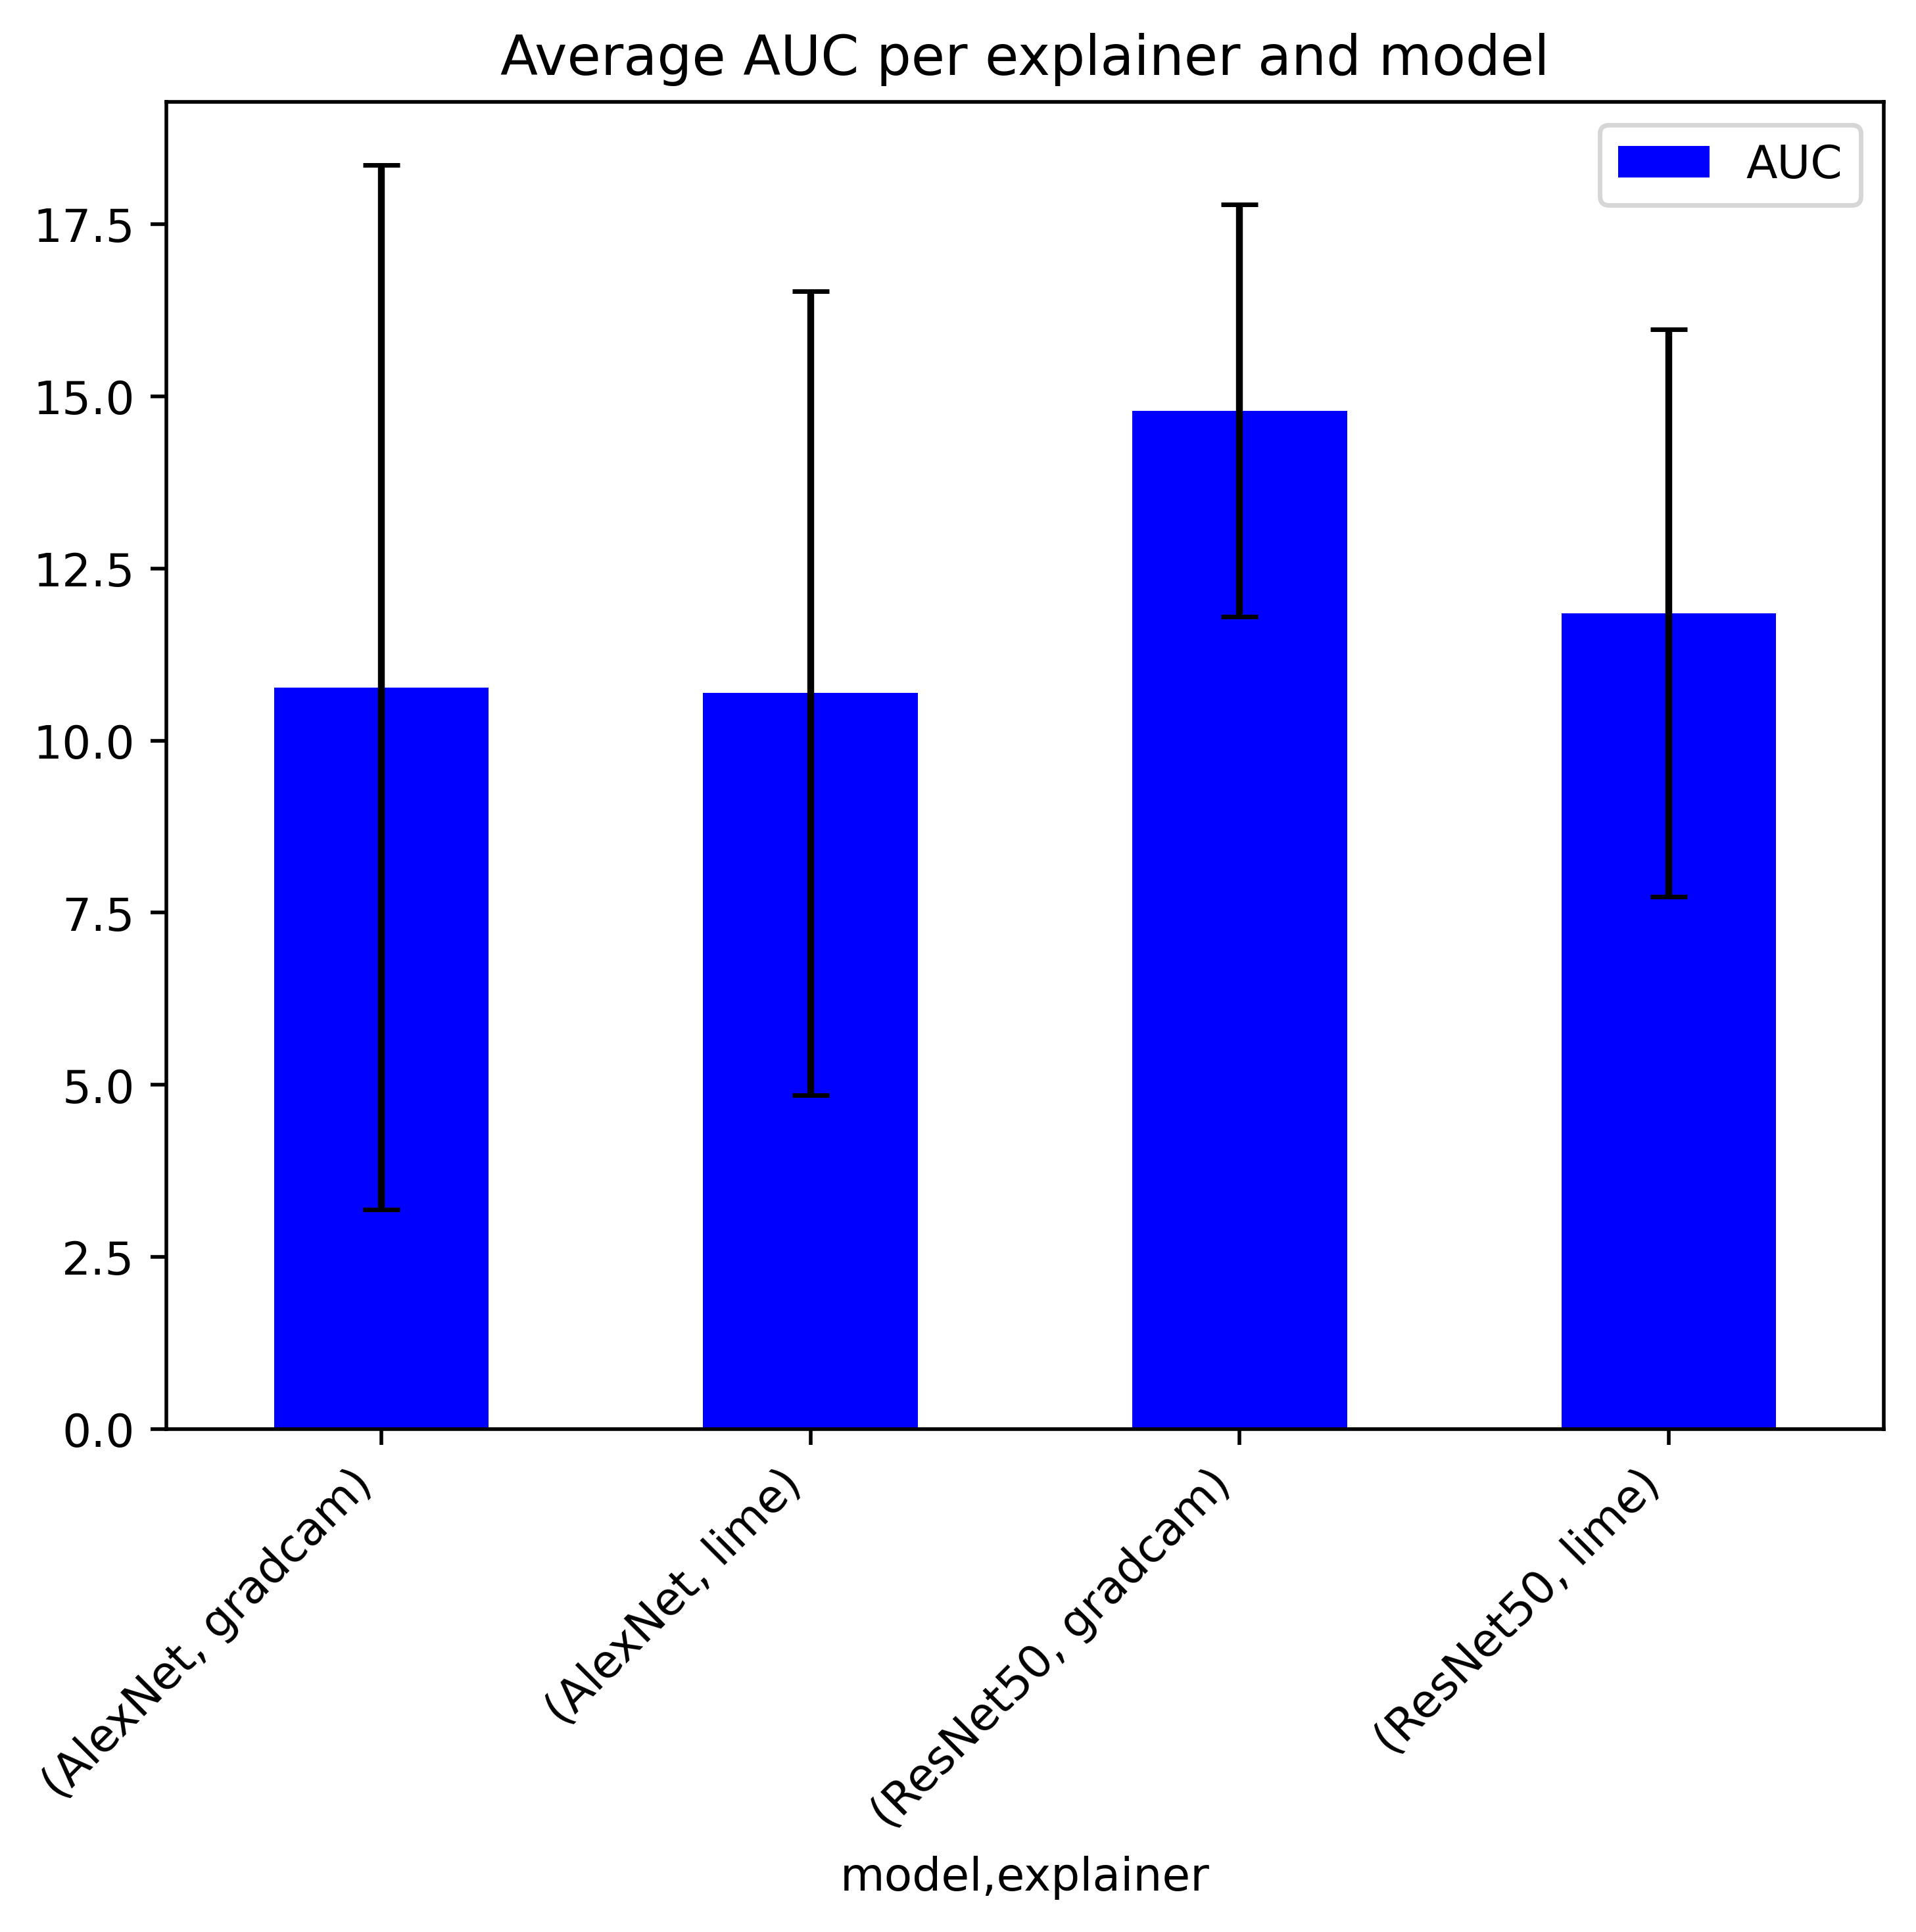
\includegraphics[width=.8\linewidth]{results/average-auc-per-exp-and-model-plus-std-dev.png}
    \caption{Average AUC values per Model and Explainer. Standard deviation shows how the AUC values vary across the entire sample set}
    \label{fig:average-auc-per-exp-and-model-plus-std-dev}
\end{figure}



% Table of average AUC scores per model and explainer
\begin{table}
    \centering
    \begin{tabular}{lll}
        \hline
        Model       & GradCAM      & LIME \\
        \hline
        AlexNet     & 10.772466    & 10.689476 \\
        ResNet50    & 14.792458    & 11.851634 \\
        \hline
    \end{tabular}
    \caption{Average AUC Score per model and explainer}
    \label{tab:plain}
\end{table}

% GradCAM highly dependent on sample image
These results suggest that LIME is generally more effective at identifying the most relevant features, as indicated by the lower AUC values, particularly on ResNet50. However, this trend does not hold universally across all instances. For example, in some cases, GradCAM significantly outperforms LIME, such as the Labrador image on AlexNet, where GradCAM achieves a much lower AUC value (approximately 2.0) compared to LIME’s 14.88 in the first run. This suggests that GradCAM’s performance can be highly dependent on the specific image being analyzed.

% Grafic 2 AUC over 10 runs for 3 sample images
\begin{figure}
    \centering
    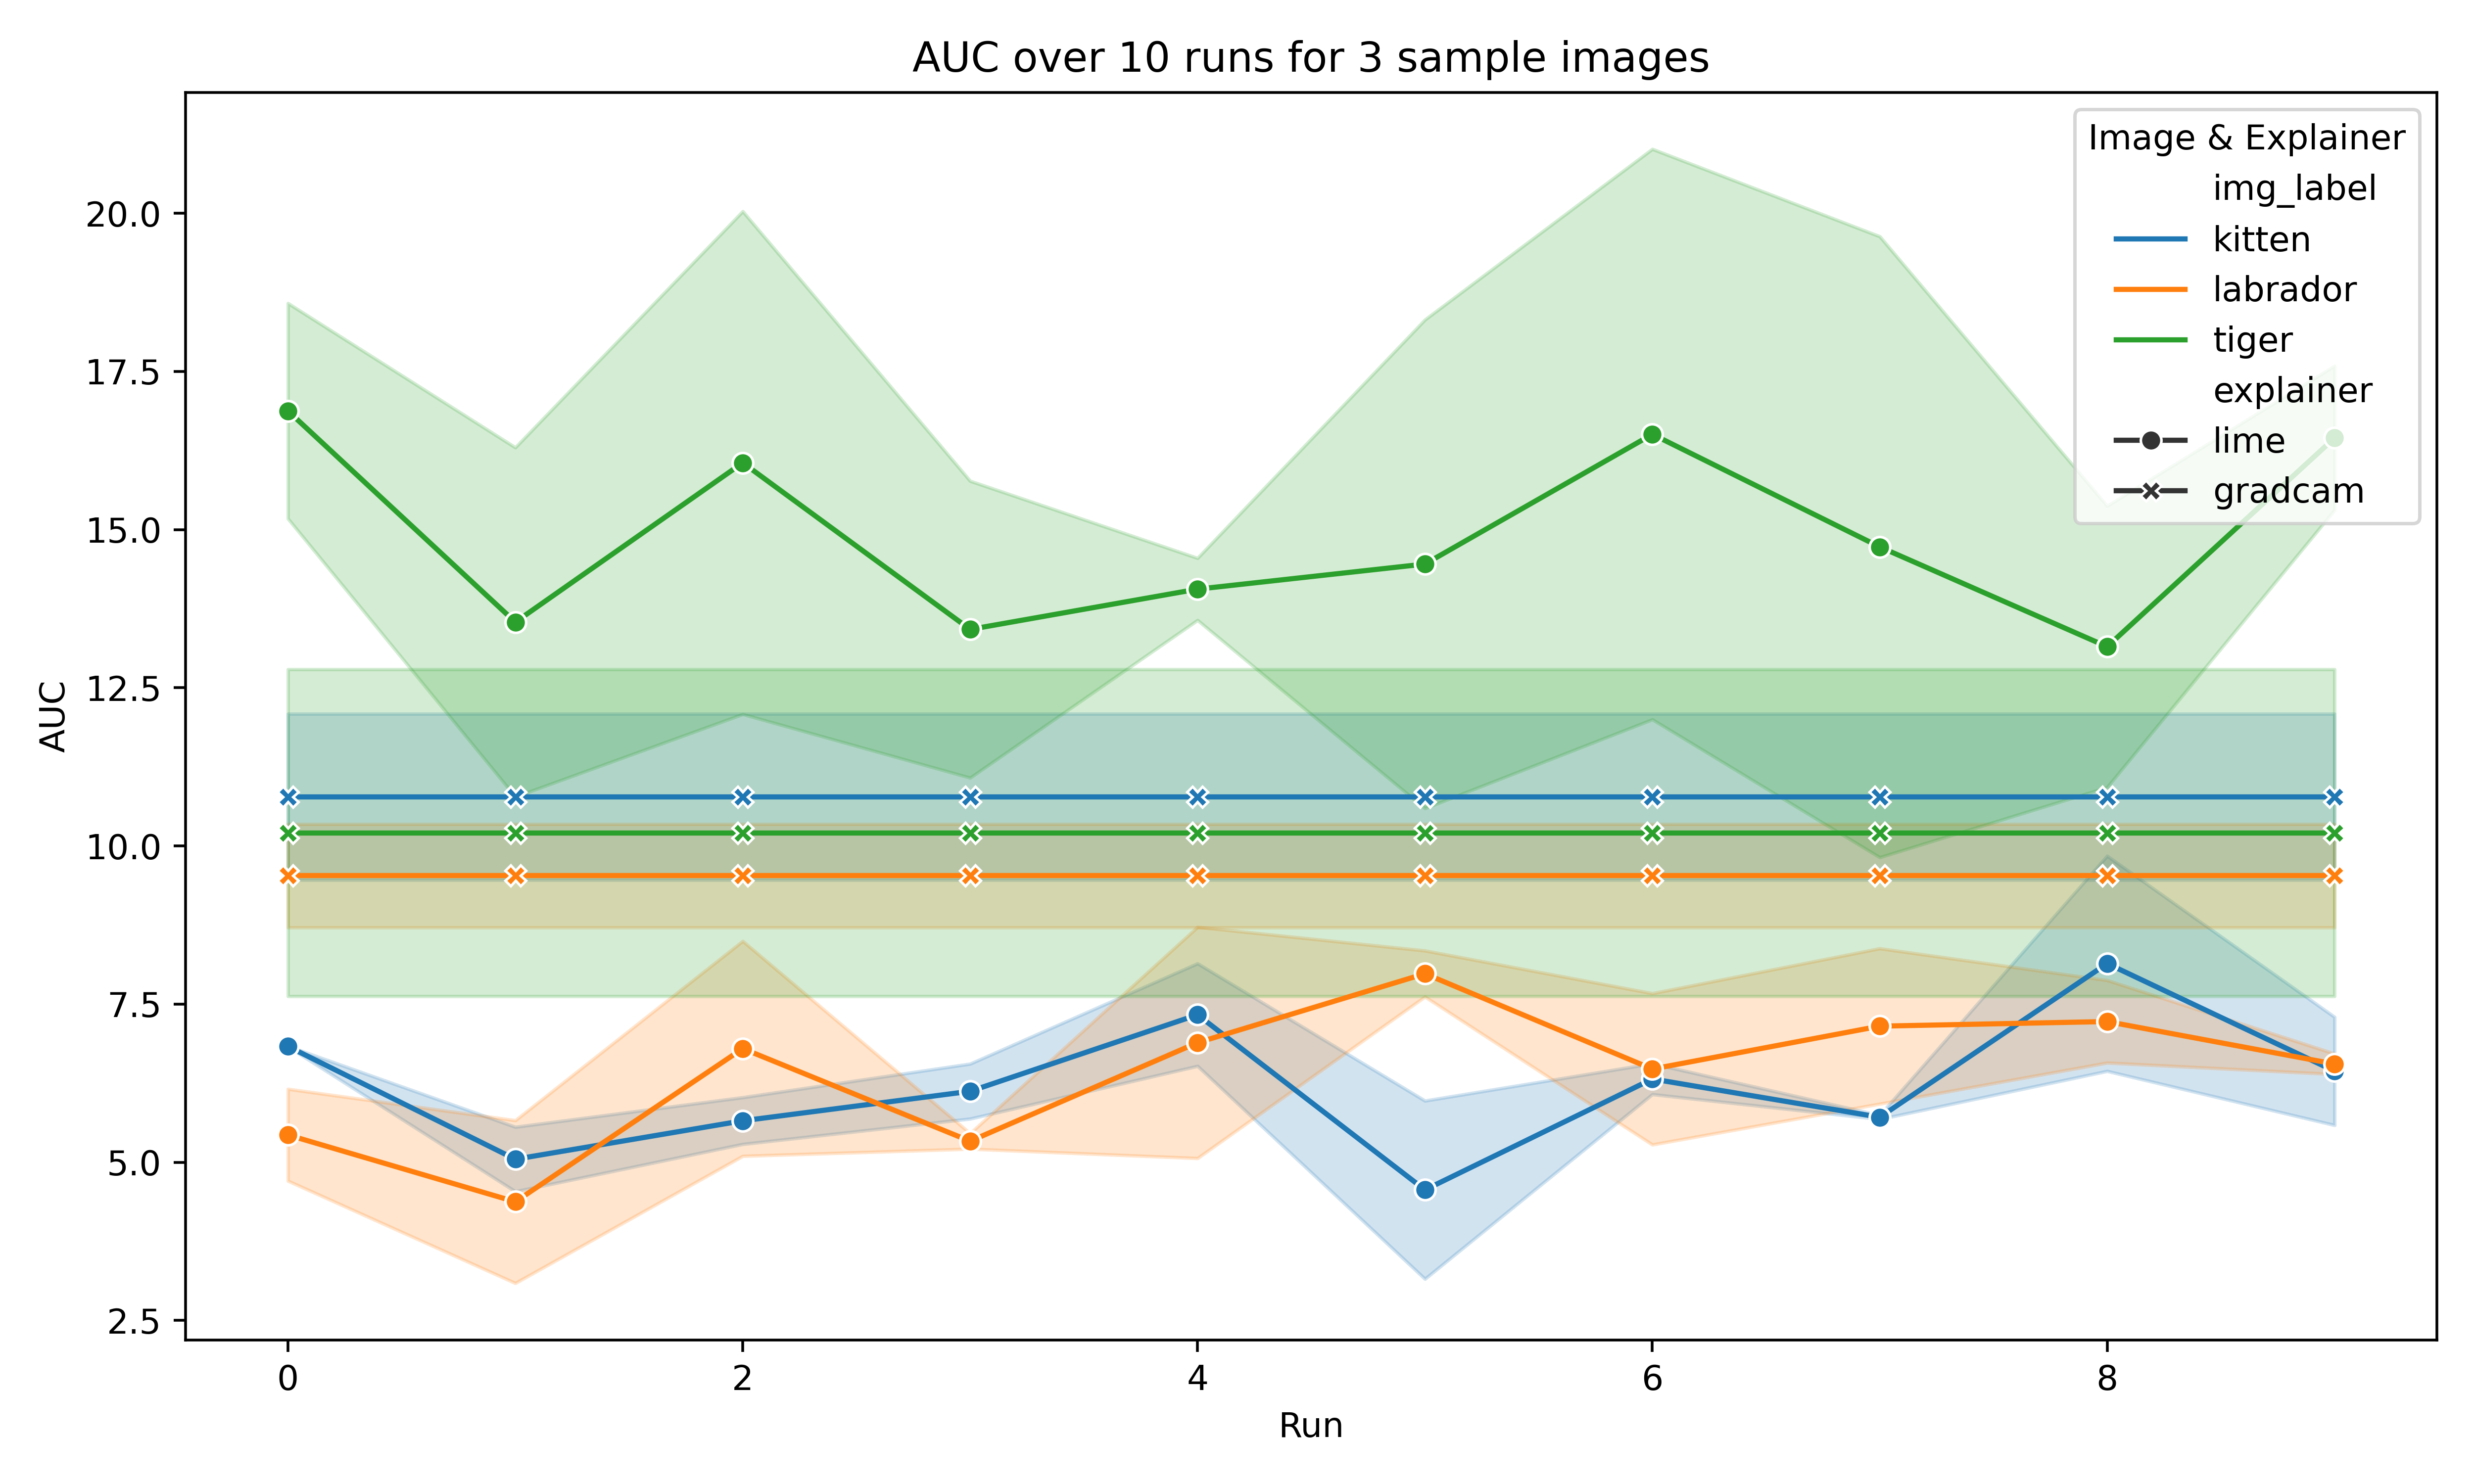
\includegraphics[width=.8\linewidth]{results/auc-over10-runs-lineplot.png}
    \caption{AUC scores over 10 runs for three sample images}
    \label{fig:auc-over10-runs-lineplot}
\end{figure}

The standard deviation of AUC values (Tables \ref{tab:table2} and \ref{tab:table3}) provides further insight into the stability of each explainer across different models. On AlexNet, GradCAM exhibits higher variance in AUC scores compared to LIME, suggesting less consistency in its explanations. Conversely, on ResNet50, GradCAM shows lower variance than LIME, highlighting the model-dependent nature of both methods’ performance.

% Table of average AUC standard deviation scores per model and explainer
\begin{table}
    \centering
    \begin{tabular}{lll}
        \hline
        Model       & GradCAM      & LIME \\
        \hline
        AlexNet     & 7.586148    & 5.835976 \\
        ResNet50    & 2.991967    & 4.118034 \\
        \hline
    \end{tabular}
    \caption{Standard deviation of average AUC per model and explainer}
    \label{tab:table1}
\end{table}

One of GradCAM’s most significant strengths lies in its deterministic nature due to its white-box approach. While LIME (a black-box method) learns a new approximation of the local explanation with each run, GradCAM produces consistent results across multiple runs. This is illustrated in Figure \ref{fig:auc-over10-runs-lineplot}, where the AUC for GradCAM remains stable across 10 runs for the same image, whereas LIME’s AUC values vary significantly. This variability in LIME’s performance, particularly when analyzing individual test instances, raises concerns about the reliability of its explanations.

%%% Standard Dev on three sample images
% AlexNet
\begin{table}
    \centering
    \begin{tabular}{lll}
        \hline
        Image       & GradCAM & LIME   \\
        \hline
        Tabby       & 0.0    &  1.789748    \\
        Labrador    & 0.0    &  1.264012    \\
        Tiger       & 0.0    &  2.343777    \\
        \hline
    \end{tabular}
    \caption{Standard deviation on three sample images per explainer on AlexNet}
    \label{tab:table2}
\end{table}

% ResNet50
\begin{table}
    \centering
    \begin{tabular}{lll}
        \hline
        Image       & GradCAM & LIME   \\
        \hline
        Tabby       & 0.0    &  0.633267    \\
        Labrador    & 0.0    &  1.256239    \\
        Tiger       & 0.0    &  2.033908    \\
        \hline
    \end{tabular}
    \caption{Standard deviation on three sample images per explainer on ResNet50}
    \label{tab:table3}
\end{table}

Overall, while LIME achieves better average AUC scores, GradCAM’s performance is more consistent across multiple runs and is highly dependent on the model being used. This trade-off between average performance and stability should be considered when choosing between the two methods, depending on the specific application and the need for reliable, repeatable explanations.

% Rückführung auf vorherige parts im Paper wichtig
\section{Discussion}
\subsection{Interpretation of Results}
% Lime vielleicht besser auf avg auc über beide modelle
% gradcam aber viel stabiler und robuster
% XAI soll Trust in AI modelle erhöhen -> Wie bewirken die beiden explainer das?
The experimental results provided valuable insights into the relative strengths and weaknesses of the two XAI methods—LIME and GradCAM—when applied to object recognition tasks. From the results, it is evident that LIME outperformed GradCAM on average AUC scores, particularly on ResNet50, where LIME achieved significantly lower AUC values. This suggests that LIME is better at focusing on the most relevant parts of an image, offering a higher degree of Explanation Selectivity across models. However, this benefit comes at the cost of stability, as LIME’s performance varies across runs due to its black-box nature.

In contrast, GradCAM displayed greater consistency and robustness across multiple runs, as seen in its minimal variance in AUC scores. This stability is a key strength, particularly in applications where repeatability is critical. While LIME’s average performance is better, GradCAM’s deterministic behavior can foster greater trust in high-stakes environments where stable and repeatable explanations are paramount.


\subsection{Application-Specific Assessment}
For the specific use case of object recognition, where understanding which parts of an image contributed to a classification is essential,  LIME’s superior average AUC performance makes it a strong contender. However, GradCAM’s robustness offers a distinct advantage in scenarios that demand consistent, model-specific explanations.

In real-world applications such as medical imaging or autonomous driving, where reliability and trust in AI models are crucial, because it can directly impact decision-making, GradCAM’s deterministic output is likely to be more advantageous. Its ability to generate consistent and repeatable explanations may lead to higher trust, particularly in fields like medicine, where understanding the rationale behind decisions is critical for both practitioners and patients. Additionally, GradCAM’s integration with the model architecture provides deeper insights into how the model arrives at its decisions, making it valuable in expert-driven fields such as pathology or robotics.

Conversely, LIME’s adaptability and model-agnostic nature make it well-suited for broader applications where the focus is on generalization across different models. For example, in applications involving rapidly changing datasets or models, such as product recommendation systems or real-time image analysis, LIME’s flexibility allows it to provide effective explanations without needing access to model internals.

Ultimately, the findings suggest that the selection of an XAI method should be guided by the specific needs of the application, balancing the trade-offs between explanation accuracy (as seen with LIME) and explanation consistency (as demonstrated by GradCAM). For high-stakes environments requiring stable, model-specific insights, white-box methods like GradCAM are preferable. For broader applications needing flexibility, black-box methods like LIME offer greater generalization and adaptability.

\subsection{Generalization of Results}

The results of this study suggest broader implications for the selection of XAI methods across various domains. While the experiments were conducted using AlexNet and ResNet50, the trade-offs between white-box and black-box methods observed here are likely applicable to other models and tasks beyond image classification.
When selecting an XAI method, it is essential to consider the context and requirements of the application. For scenarios where consistency and model-specific insights are critical—such as in regulated industries or research environments—white-box methods like GradCAM provide significant advantages. GradCAM’s internal knowledge of the model’s architecture allows it to offer stable and transparent explanations that enhance user trust.

On the other hand, black-box methods like LIME may be preferable in applications that demand flexibility and generalization across different models. LIME’s ability to provide explanations for any model makes it a versatile tool, especially in dynamic environments where AI systems are frequently updated or retrained.

%% The file named.bst is a bibliography style file for BibTeX 0.99c



\appendix

\section*{Acknowledgments}

I sincerely thank my supervisor, Dr. Gesina Schwalbe, for her unwavering guidance and support throughout this research project. I am deeply grateful for her valuable feedback, thoughtful suggestions, and the immense amount of time she dedicated to ensuring we truly understood the subject. This Project has reignited my enthusiasm for Artificial Intelligence and provided me with profound insights into the world of professional research. This project would not have been possible without her dedication and contributions.

\section*{Application of Explanation Selectivity}

Figure 3 illustrates the feature removal process for GradCAM on AlexNet using the labrador test image. The heatmap generated by GradCAM highlights the dog’s face as the most important feature, which is consistent with the model’s classification. The AUC score for this instance is shown in Figure 4, indicating the effectiveness of GradCAM in identifying the key features for the model’s prediction. Additionally, Figure 5 demonstrates the feature removal process for LIME on ResNet50 using the tabby test image. LIME generates a local explanation around the instance being explained, highlighting the features that are most influential for the model’s prediction. The AUC score for this instance is shown in Figure 6, providing insights into LIME’s performance in identifying the key features for the model’s decision-making process.

\begin{figure}
    \centering
    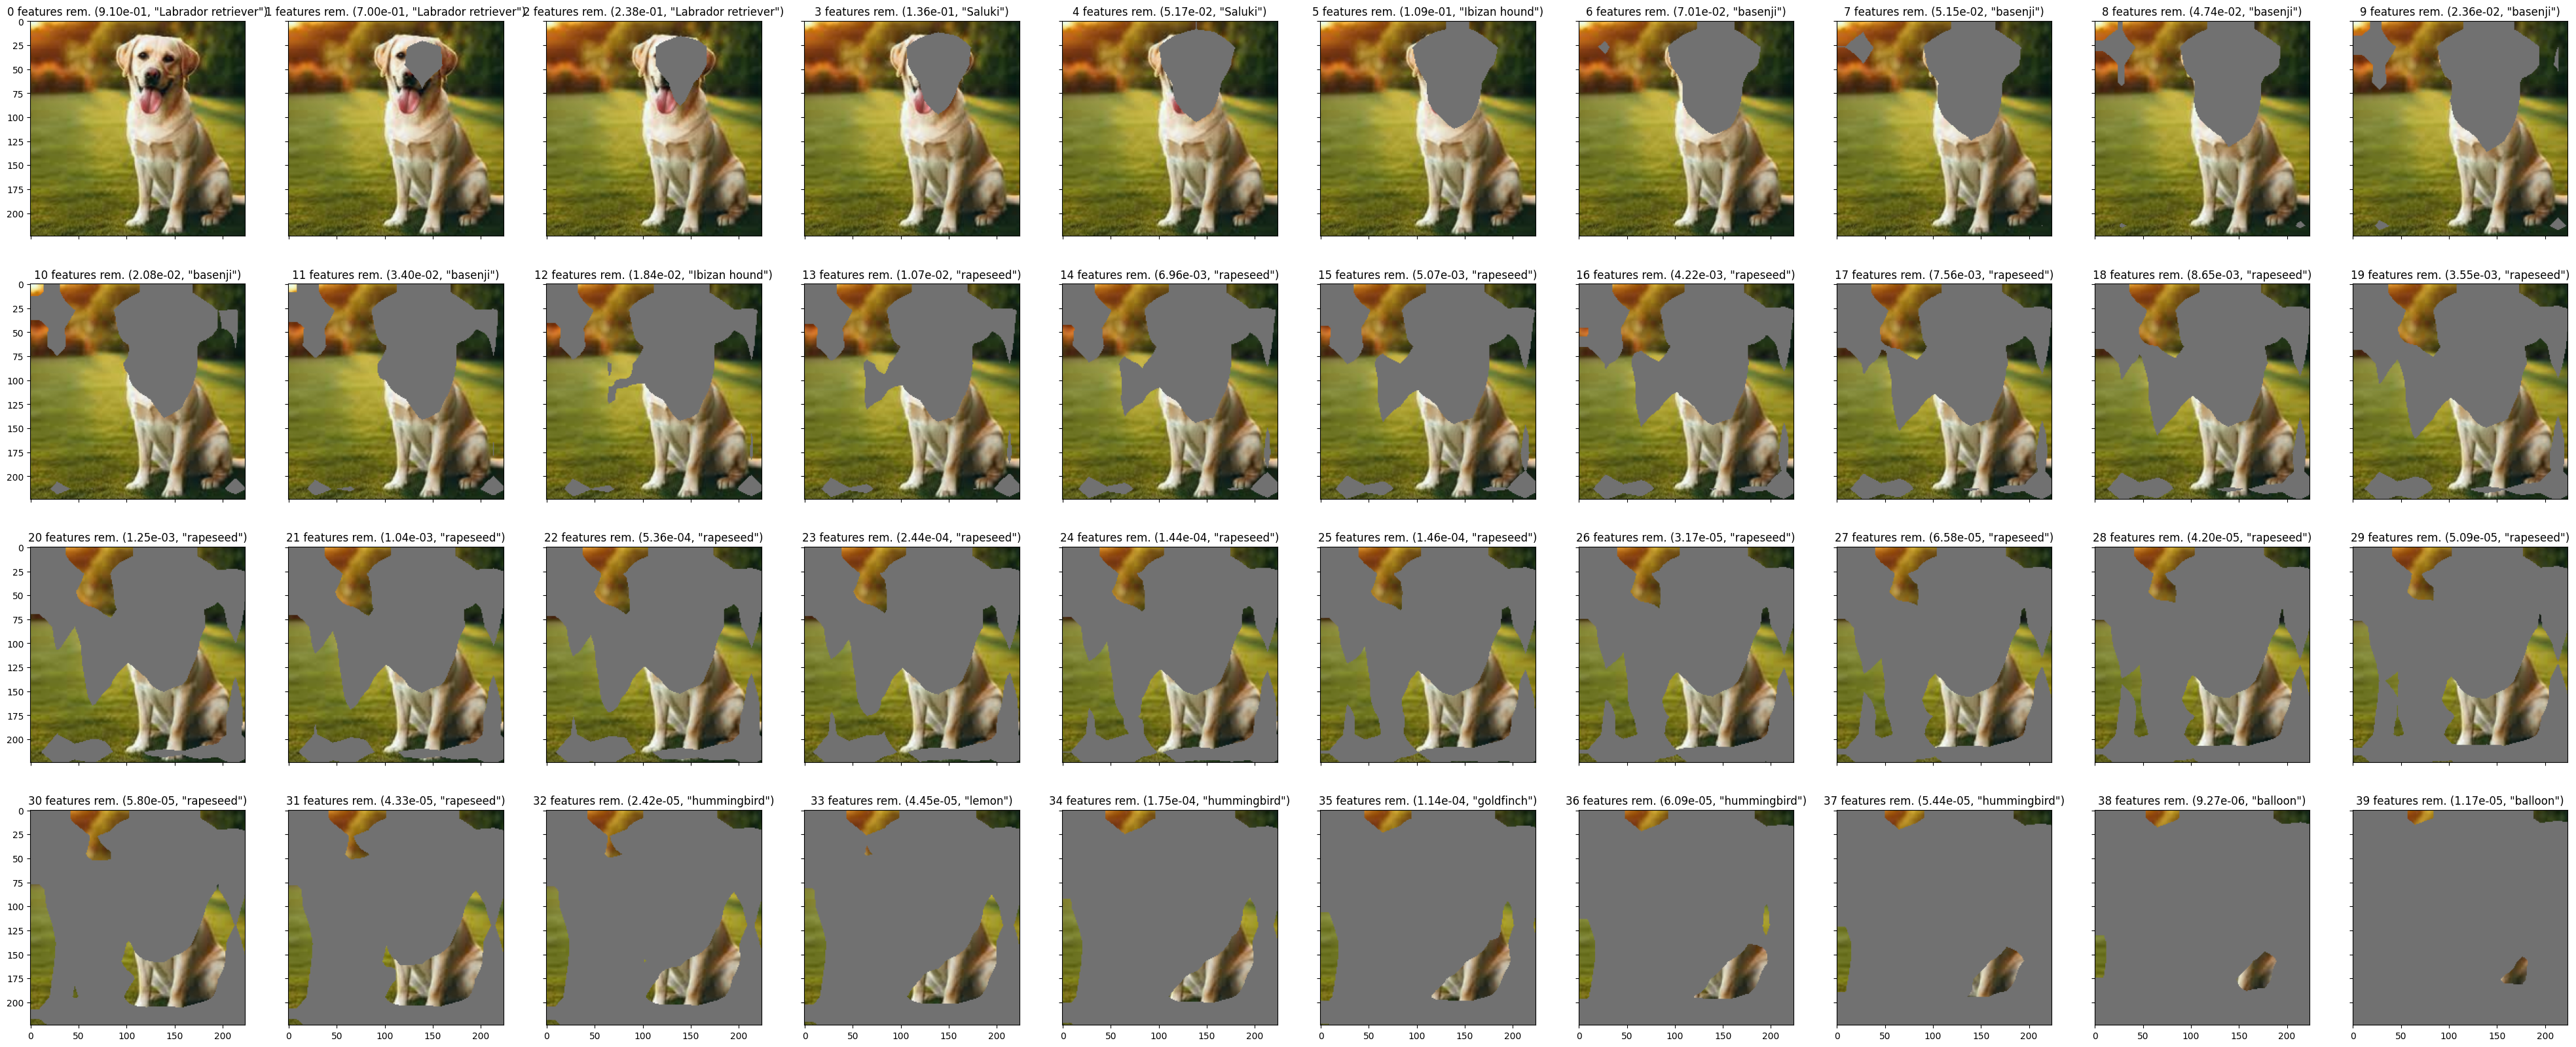
\includegraphics[width=1\linewidth]{results/gradcam-labrador-feature-removal.png}
    \caption{GradCAM on AlexNet. Notice how it correctly identifies the dog's face as most important feature.}
    \label{fig:gradcam-labrador-feature-removal}
\end{figure}


\begin{figure}
    \centering
    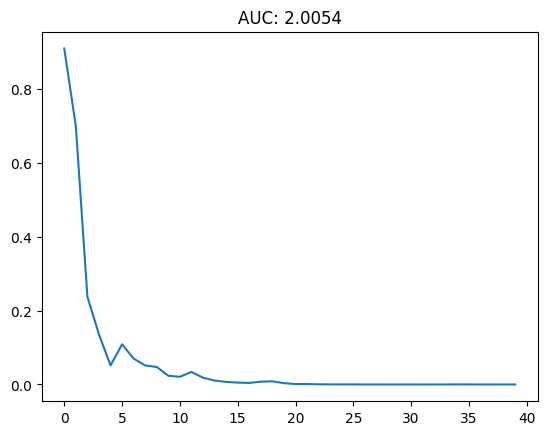
\includegraphics[width=1\linewidth]{results/gradcam-labrador-auc.png}
    \caption{AUC score for GradCAM on AlexNet for labrador test image}
    \label{fig:gradcam-labrador-auc}
\end{figure}


\begin{figure}
    \centering
    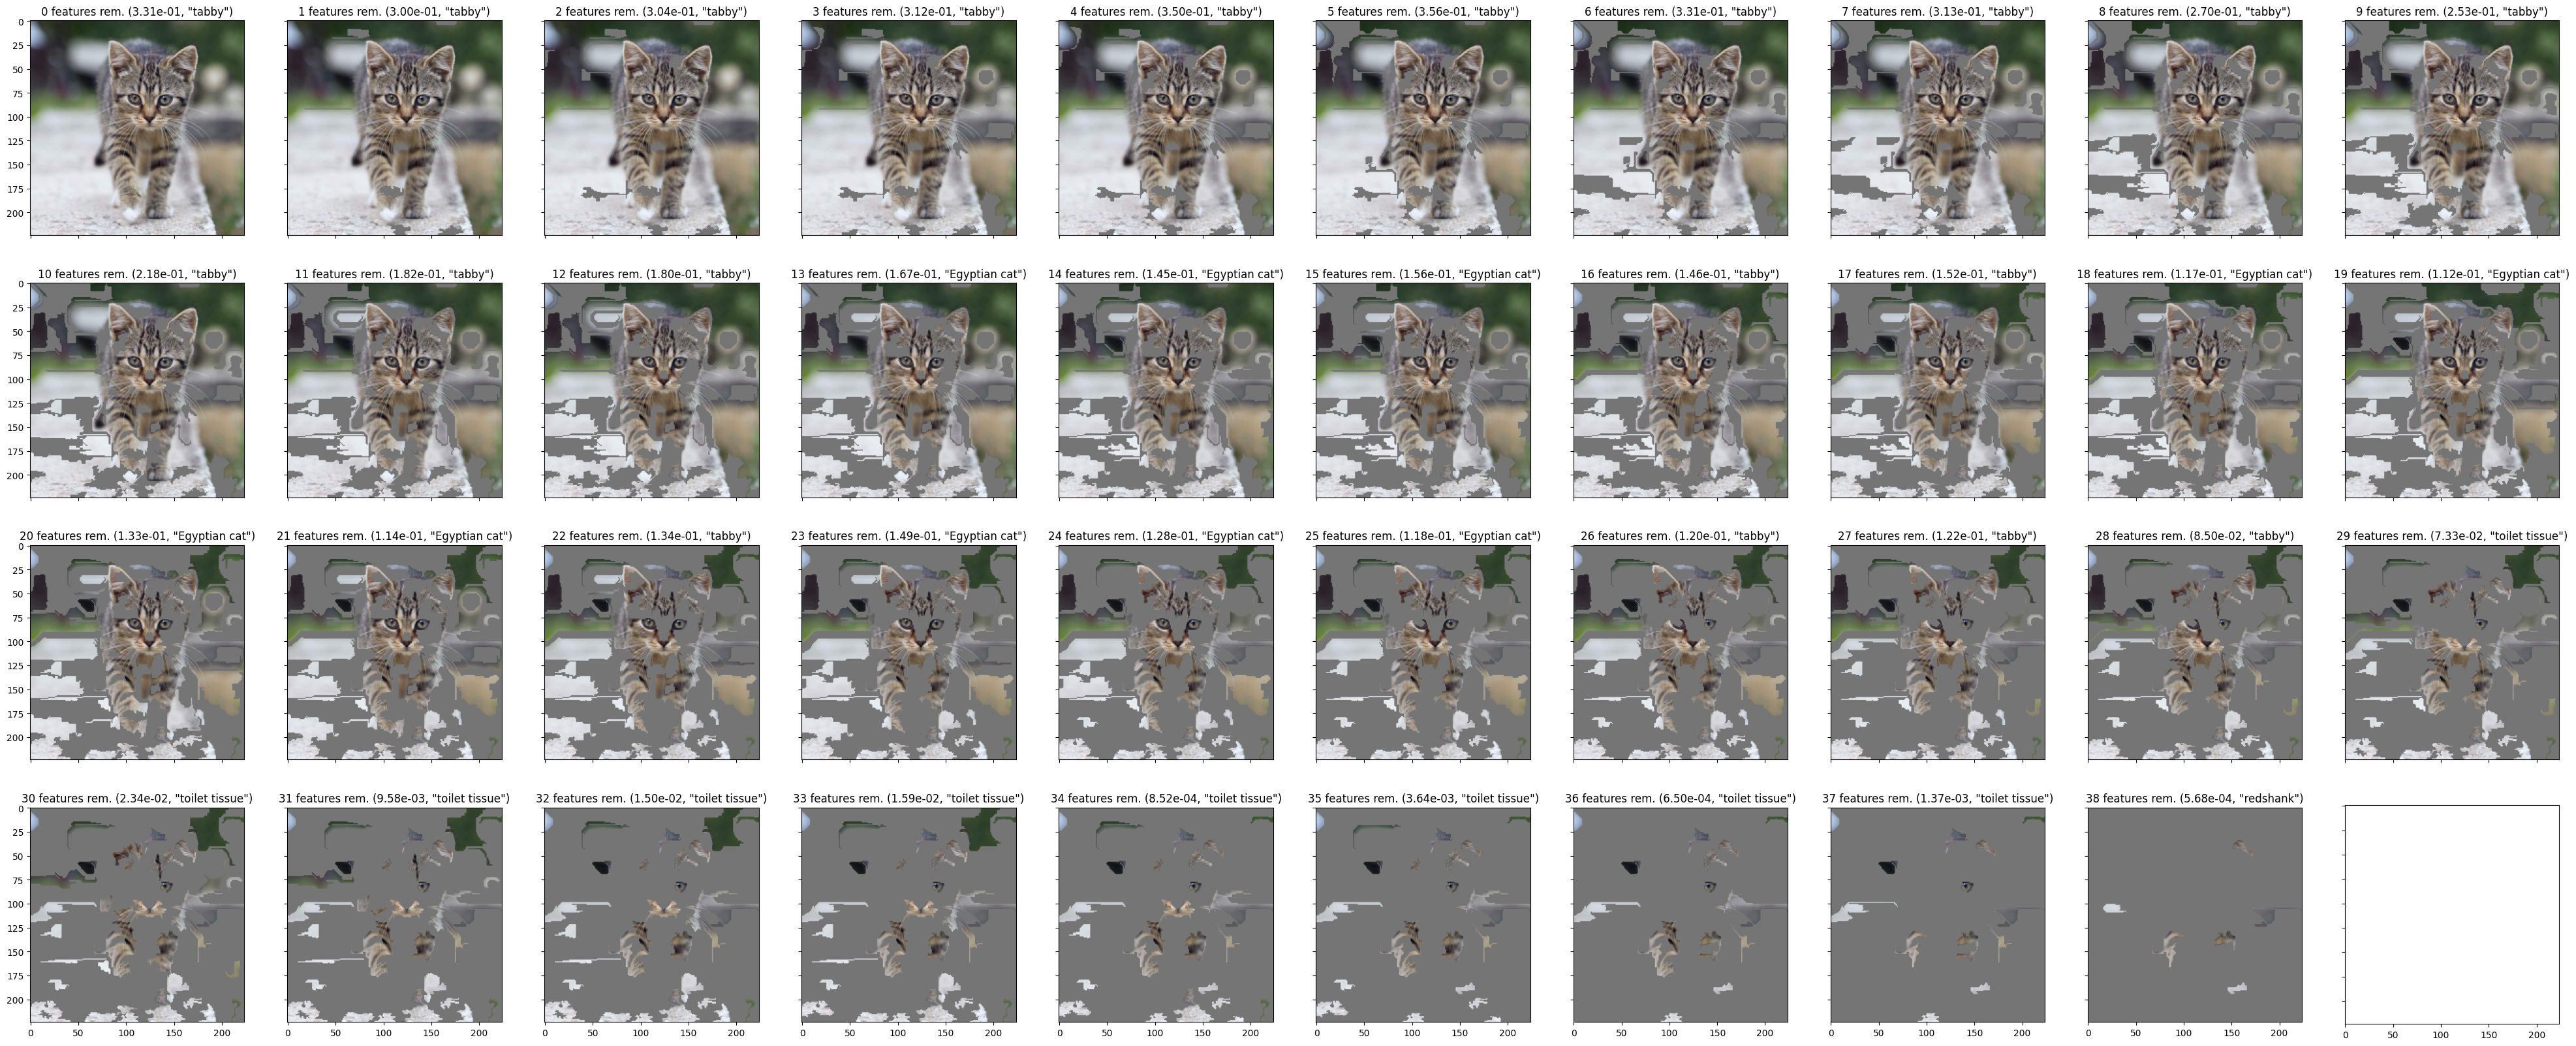
\includegraphics[width=1\linewidth]{results/lime-tabby-feature-removal.png}
    \caption{LIME on ResNet50. LIME learns a local explanation around the instance being explained.}
    \label{fig:lime-tabby-feature-removal}
\end{figure}


\begin{figure}
    \centering
    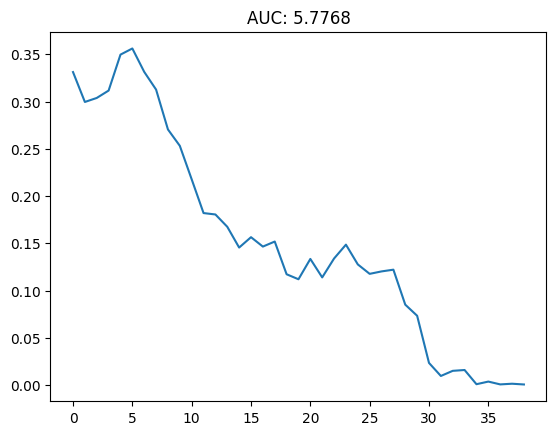
\includegraphics[width=1\linewidth]{results/lime-tabby-auc.png}
    \caption{AUC score for LIME on ResNet for cat test image}
    \label{fig:lime-tabby-auc}
\end{figure}

\bibliographystyle{named}
\bibliography{ijcai24}

\end{document}
